\begin{center}
    \Large \textbf{Hinweise zur Klausur}
\end{center}
Achte darauf, dass du auf jedem Blatt auf dem Antwortbogen deine Startnummer gut lesbar im dafür vorgesehenen Kästchen notierst. Lies dir zu Beginn alle Aufgaben gründlich durch. Viel Erfolg!

\begin{center}
    \Large \textbf{Periodensystem}
    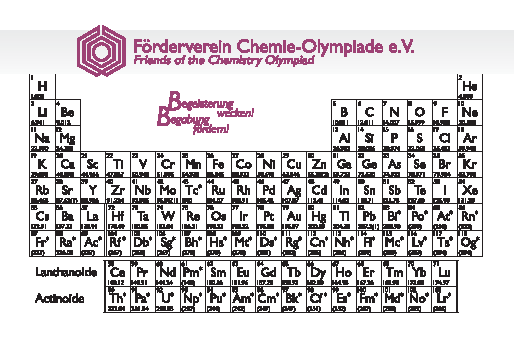
\includegraphics[page=1, scale=2.5, angle=270]{Format_Material/PSE.pdf}
\end{center}

\newpage
\section*{Formelsammlung}
\subsection*{wichtige chemische und physikalische Konstanten}
\begin{table}[H]
\renewcommand{\arraystretch}{1.3}
    \begin{tabular}{p{7cm} l}
        Elementarladung &  $e = \SI{1.602176e-19}{\coulomb}$\\
        Universelle Gaskonstante & $R = \SI{8,314456}{\joule\per\mol\per\kelvin}$\\
        Avogadro-Konstante & $N_\mathrm{A} = \SI{6,0221e23}{\per\mol}$\\
        Faraday Konstante & $F = \SI{96485,309}{\coulomb\per\mol}$\\
        Atomare Masseneinheit & $u =$ \SI{1,660539e-27}{\kilo\gram}\\
        Planck'sches Wirkungsquantum & $h = \SI{6.62607015E-34}{\joule\second}$\\
        Lichtgeschwindigkeit & $c = $ \SI{2.99792458e8}{\meter\per\second}
    \end{tabular}
\end{table}

\subsection*{Allgemeine Gleichungen}

\begin{table}[H]
\renewcommand{\arraystretch}{1.3}
    \begin{tabular}{p{7cm} l}
       ideales Gasgesetz & $p V = n R T$\\
       radioaktives Zerfallsgesetz & $N(t) = N(0) e^{-k t} = N(0) e^{-\frac{\ln 2}{T_{1/2}} t}$\\
    \end{tabular}
\end{table}

\subsection*{Gleichgewichte}

\begin{table}[H]
\renewcommand{\arraystretch}{1.3}
    \begin{tabular}{p{7cm} l}
       Massenwirkungsgesetz & $K_\mathrm{c} = \frac{c(\mathrm{C})^c \cdot c(\mathrm{D})^d \cdot \dots}{c(\mathrm{A})^a \cdot c(\mathrm{B})^b \cdot \dots}$\\
       Säure-Base-Gleichgewichte & $K_\mathrm{S} = \frac{c(\mathrm{H^+}) \cdot c(\mathrm{A^-})}{c(\mathrm{HA}) \cdot c_0}$\\
       & $K_\mathrm{B} = \frac{c(\mathrm{HB^+}) \cdot c(\mathrm{OH^-})}{c(\mathrm{B})\cdot  c_0}$\\
       pH-Wert & $\mathrm{pH} = - \log \frac{c(\mathrm{H^+})}{c_0}$\\
       Henderson-Hasselbalch & $\mathrm{pH} = \mathrm{p}K_\mathrm{S} + \log \frac{c(\ce{A-})}{c(\ce{HA})}$\\
    \end{tabular}
\end{table}

\subsection*{Thermodynamik und Elektrochemie}

\begin{table}[H]
\renewcommand{\arraystretch}{1.3}
    \begin{tabular}{p{7cm} l}
       Gibbs-Helmholtz-Gleichung & $\Delta G_\mathrm{R}^\circ = \Delta H_\mathrm{R}^\circ - T \Delta S_\mathrm{R}^\circ$\\
      Gibbs-Energie und Gleichgewichtskonstante & $\Delta G_\mathrm{R}^\circ = - R T \ln K$\\
       Faradaysches Gesetz & $Q = I \cdot t = z \cdot n \cdot F$
    \end{tabular}
\end{table}